%% ============================================================
%% TRIX: Training-Free Reranking for Instruction-Following Retrieval with Exclusions
%%
%% Target: AAAI 2027
%% Format: AAAI two-column LaTeX
%% ============================================================

\documentclass[letterpaper]{article}
\usepackage[submission]{aaai2027}
\usepackage[hyphens]{url}
\usepackage{graphicx}
\urlstyle{rm}
\def\UrlFont{\rm}
\usepackage{natbib}
\usepackage{caption}
\frenchspacing

% ============================================================
% Additional packages (compatible with aaai2027)
% ============================================================
\usepackage{amsmath}
\usepackage{amssymb}
\usepackage{booktabs}
\usepackage{multirow}
\usepackage{xspace}

% ============================================================
% Custom macros
% ============================================================
\newcommand{\method}{\ifmmode \mathrm{TRIX}\else TRIX\xspace\fi}
\newcommand{\qbase}{Q_{\text{full}}}
\newcommand{\qpos}{Q_{\text{pos}}}
\newcommand{\qneg}{Q_{\text{neg}}}
\newcommand{\qplus}{Q_{+}}
\newcommand{\qminus}{Q_{-}}
\newcommand{\sbase}{S_{\text{full}}}
\newcommand{\spos}{S_{\text{pos}}}
\newcommand{\sneg}{S_{\text{neg}}}
\newcommand{\sfinal}{S_{\text{final}}}

\pdfinfo{
/TemplateVersion (2027.1)
}

\setcounter{secnumdepth}{2}

% ============================================================
% Author info (anonymous submission)
% ============================================================
\title{TRIX: Training-Free Reranking for Instruction-Following Retrieval with Exclusions}
\author{
    Anonymous Submission
}
\affiliations{}

\begin{document}

\maketitle

% ============================================================
% ABSTRACT
% ============================================================
\begin{abstract}
Retrieval requests often combine a target topic with positive criteria,
background context, and explicit exclusions.  Frozen retrievers rely heavily on
lexical and semantic entity matching, overlooking how these instructions
define relevance.  This failure is acute for exclusions, where an excluded
entity can become a strong matching signal.  Existing remedies often require
instruction training or representation adaptation.  We introduce \method{}, a
training-free reranking framework for frozen retrievers.  \method{} preserves
the complete request for retrieval and decomposes it into affirmative and
exclusion views, focusing positive evidence and removing irrelevant background
context.  The two views can still share topic information, causing raw
exclusion scores to penalize relevant content.  \method{} removes the exclusion
similarity predicted by affirmative relevance, then uses the residual to reduce
positive scores and suppress exclusion matches.  It requires no model
training, retriever updates, or document re-encoding.  Across three benchmarks
and six frozen retrievers, \method{} improves retrieval effectiveness and
instruction sensitivity, increasing the latter by up to 16.4 points and
outperforming a matched training-free baseline on NegConstraint by up to
3.4 points.
\end{abstract}

% ============================================================
% 1. INTRODUCTION
% ============================================================
\section{Introduction}
\label{sec:introduction}

Retrieval requests often combine a target topic with positive relevance
criteria, background context, and explicit exclusions.  Frozen retrievers rely
mainly on lexical and semantic matching, but these signals do not reliably
capture how each part of an instruction affects relevance.  The problem is
especially clear for exclusions because the excluded entity remains part of
the request.  In lexical retrieval, it contributes matching terms like any
other query content.  Dense retrievers face a related limitation: pooled
embeddings compress topical content and compositional roles into a single
vector, and cosine scoring can keep texts with similar content but different
negation or scope close in the embedding space
\cite{DBLP:journals/corr/abs-2604-16351}.  A document can therefore receive a
higher score for matching an entity that the user explicitly asks to exclude.
Figure~\ref{fig:trix-overview} illustrates a request for evidence that a US
college education improves employment or income while excluding documents
about Manhattan colleges such as Columbia University.  Documents about
employment outcomes for Columbia graduates match the topic and entities in the
request, yet they violate the exclusion.  This failure is consistent with prior
findings that neural rankers often fail to adjust their rankings when negation
changes the relevance conditions
\cite{DBLP:conf/eacl/WellerLD24,DBLP:conf/naacl/WellerCMLCDLS25}.

Separating the instruction into positive and exclusion views is a natural way
to make these roles explicit.  However, the two views can still share topic
information.  In Figure~\ref{fig:trix-overview}, the fifth-ranked document
satisfies the request and does not discuss the excluded Manhattan colleges,
but retrieval scores are based mainly on lexical or embedding similarity.
Its broader discussion of US colleges and graduate outcomes therefore raises
its scores under both the affirmative and exclusion views.  Directly
subtracting the exclusion score would penalize a relevant document.  An
effective correction must distinguish evidence of the excluded content from
similarity caused by the shared topic.

Prior methods introduce instruction control through instruction-trained
retrieval, inference-time query adaptation, or logic-based constraint
modeling.  Instruction-trained retrievers such as Promptriever
\cite{DBLP:conf/iclr/WellerDLPZH25}, Dual-View Training \cite{dualview2026}, and
InstEmb \cite{gao2026instemb} learn instruction-conditioned representations,
but require additional supervision and model training.  Inference-time query
adaptation methods such as DEO
\cite{DBLP:journals/corr/abs-2603-09185} modify the query embedding at
inference time, but direct optimization can move the query vector away from
the embedding structure learned by the retriever, making its similarity to
document embeddings less reliable.  Logic-based constraint methods such as NS-IR
\cite{xu2025logical} and OrLog \cite{hoveyda2026orlog} translate instructions
into logical structures and apply symbolic or probabilistic inference over the
retrieved candidates.  The additional translation, candidate-level model
calls, and formal inference increase online retrieval latency.

We therefore introduce \method, a training-free reranking framework that
corrects the scores of a frozen retriever without updating its representations,
re-encoding documents, or adding candidate-level constraint inference.
\method retains the complete instruction for initial retrieval, derives an
affirmative view that focuses the positive criteria and removes irrelevant
background context, and represents excluded content in a separate view.  It
uses a query-local residual as a proxy for exclusion evidence beyond topical
match.  Based on this signal, the final scoring rule preserves or reduces
affirmative support and applies an exclusion penalty.

Across an instruction-following benchmark (FollowIR) and two exclusion-aware
benchmarks (NegConstraint and ExcluIR), \method improves instruction-aware
ranking across sparse and dense frozen retrievers.  It raises instruction
sensitivity by up to 16.4 points and outperforms a matched training-free
baseline on NegConstraint by up to 3.4 points.

Our contributions are:
\begin{itemize}
    \item[$\bullet$] We introduce a training-free reranking framework that uses full,
    affirmative, and exclusion views to handle positive criteria, background
    context, and exclusions without retriever updates or document re-encoding.
    \item[$\bullet$] We use residual correction to obtain a query-local proxy
    for exclusion evidence beyond topical match, then combine relevance
    promotion and exclusion suppression according to this signal.
    \item[$\bullet$] Across three benchmarks and multiple frozen retrievers, we
    demonstrate consistent improvements and isolate the effects of view
    construction, residual scoring, and final score correction, while
    maintaining general retrieval effectiveness.
\end{itemize}

% ============================================================
% 2. RELATED WORK
% ============================================================
\section{Related Work}
\label{sec:related-work}

Prior work on instruction control in retrieval falls into three groups:
instruction-trained retrieval, inference-time query adaptation, and logic-based
constraint modeling.

\subsection{Instruction-Trained Retrieval}

Instruction-trained retrievers learn to score documents according to
natural-language instructions.
TART uses multitask instruction tuning with natural-language task descriptions
\cite{DBLP:conf/acl/AsaiSL0I0HY23}.
INSTRUCTOR learns a shared instruction-conditioned embedding space
\cite{DBLP:conf/acl/SuSKWHOYSZ023}.  HypeR composes task-dependent prompts for
cross-domain retrieval \cite{DBLP:conf/iclr/CaiT0XGL0J23}.  More recent systems
train directly with relevance instructions, including FollowIR-7B
\cite{DBLP:conf/naacl/WellerCMLCDLS25}, Promptriever
\cite{DBLP:conf/iclr/WellerDLPZH25},
and InF-IR \cite{zhuang2025infir}.  Dual-View Training adds
polarity-reversed supervision \cite{dualview2026}, while InstEmb combines
input-intrinsic and output-aware signals when learning instruction-following
embeddings \cite{gao2026instemb}.  CoDeR learns constraint compatibility
through polarity supervision, requiring an additional trained encoder and
corpus re-encoding \cite{DBLP:journals/corr/abs-2606-13204}.

These training-based methods require instruction-specific data and updates to
the retriever parameters.  Targeted negation augmentation likewise requires
additional training data \cite{DBLP:conf/emnlp/SinghKS23}, and supporting new
instruction types can require further data and retraining.  \method{} keeps the
retriever and its representation function fixed and introduces instruction
control during reranking.

\subsection{Inference-Time Query Adaptation}

Inference-time methods modify the query text or representation without
retraining the retriever \cite{DBLP:conf/emnlp/MaGHZD23}.
HyDE generates a hypothetical document to guide retrieval
\cite{DBLP:conf/acl/GaoMLC23}.  Query2Doc expands the query with a generated
pseudo-document \cite{DBLP:conf/emnlp/WangYW23}.  RAG-Fusion combines rankings
from multiple generated queries \cite{raudaschl2024ragfusion}.  Stage-Aware
Decomposition retains the complete query for initial retrieval and additively
aggregates decomposed condition scores during reranking
\cite{yin2026stageaware}.  These methods add or reformulate topical content but
do not handle exclusion constraints.  Excluded entities can therefore remain
strong lexical or semantic matching signals.

Other methods directly modify or construct query representations.  DEO derives
positive and negative subqueries and optimizes the query embedding toward the
former and away from the latter
\cite{DBLP:journals/corr/abs-2603-09185}.  Because the resulting vector
is not generated by the retriever's query encoder, it may deviate from the
learned embedding structure and make its similarity to document embeddings
less reliable.  In vision--language retrieval,
SpaceVLM-DRC uses
angular composition to construct three negation-aware query directions and
combines their image similarities with a direct image-space repulsion term
\cite{pokhrel2026negation}.  This design assumes a unit-normalized shared
image--text embedding space and treats direct similarity to the negated
concept as evidence that an image contains it.  Text retrieval therefore
requires a scoring rule that supports sparse retrievers and distinguishes
exclusion evidence from similarity caused by shared topic information.

\method{} formulates instruction control as score correction over the
retrieved documents.  It retains the complete query for candidate retrieval,
keeps the query and document representations unchanged, estimates exclusion
evidence from the relation between affirmative and exclusion scores, and
combines relevance promotion with exclusion suppression.  This score-based
formulation applies to sparse and dense text retrievers.

\subsection{Logic-Based Constraint Modeling}

Logic-based methods represent constraints explicitly before reranking.
NS-IR translates queries and documents into first-order logic and combines
semantic alignment with connective constraints for negative-constraint
retrieval \cite{xu2025logical}.  OrLog decomposes entity-seeking queries into
atomic predicates and a logical form, then uses predicate plausibility scores
in probabilistic logic inference \cite{hoveyda2026orlog}.

These methods enforce constraint composition through formal representations
and candidate-level inference.  The required logical translation, model calls,
and formal inference increase online latency and make retrieval depend on the
quality of the intermediate logical representation.  \method{} operates
directly on the scores of a frozen retriever, without translating documents
into logical forms or invoking an external inference engine.

% ============================================================
% 3. METHODOLOGY
% ============================================================
\begin{figure*}[t]
\centering
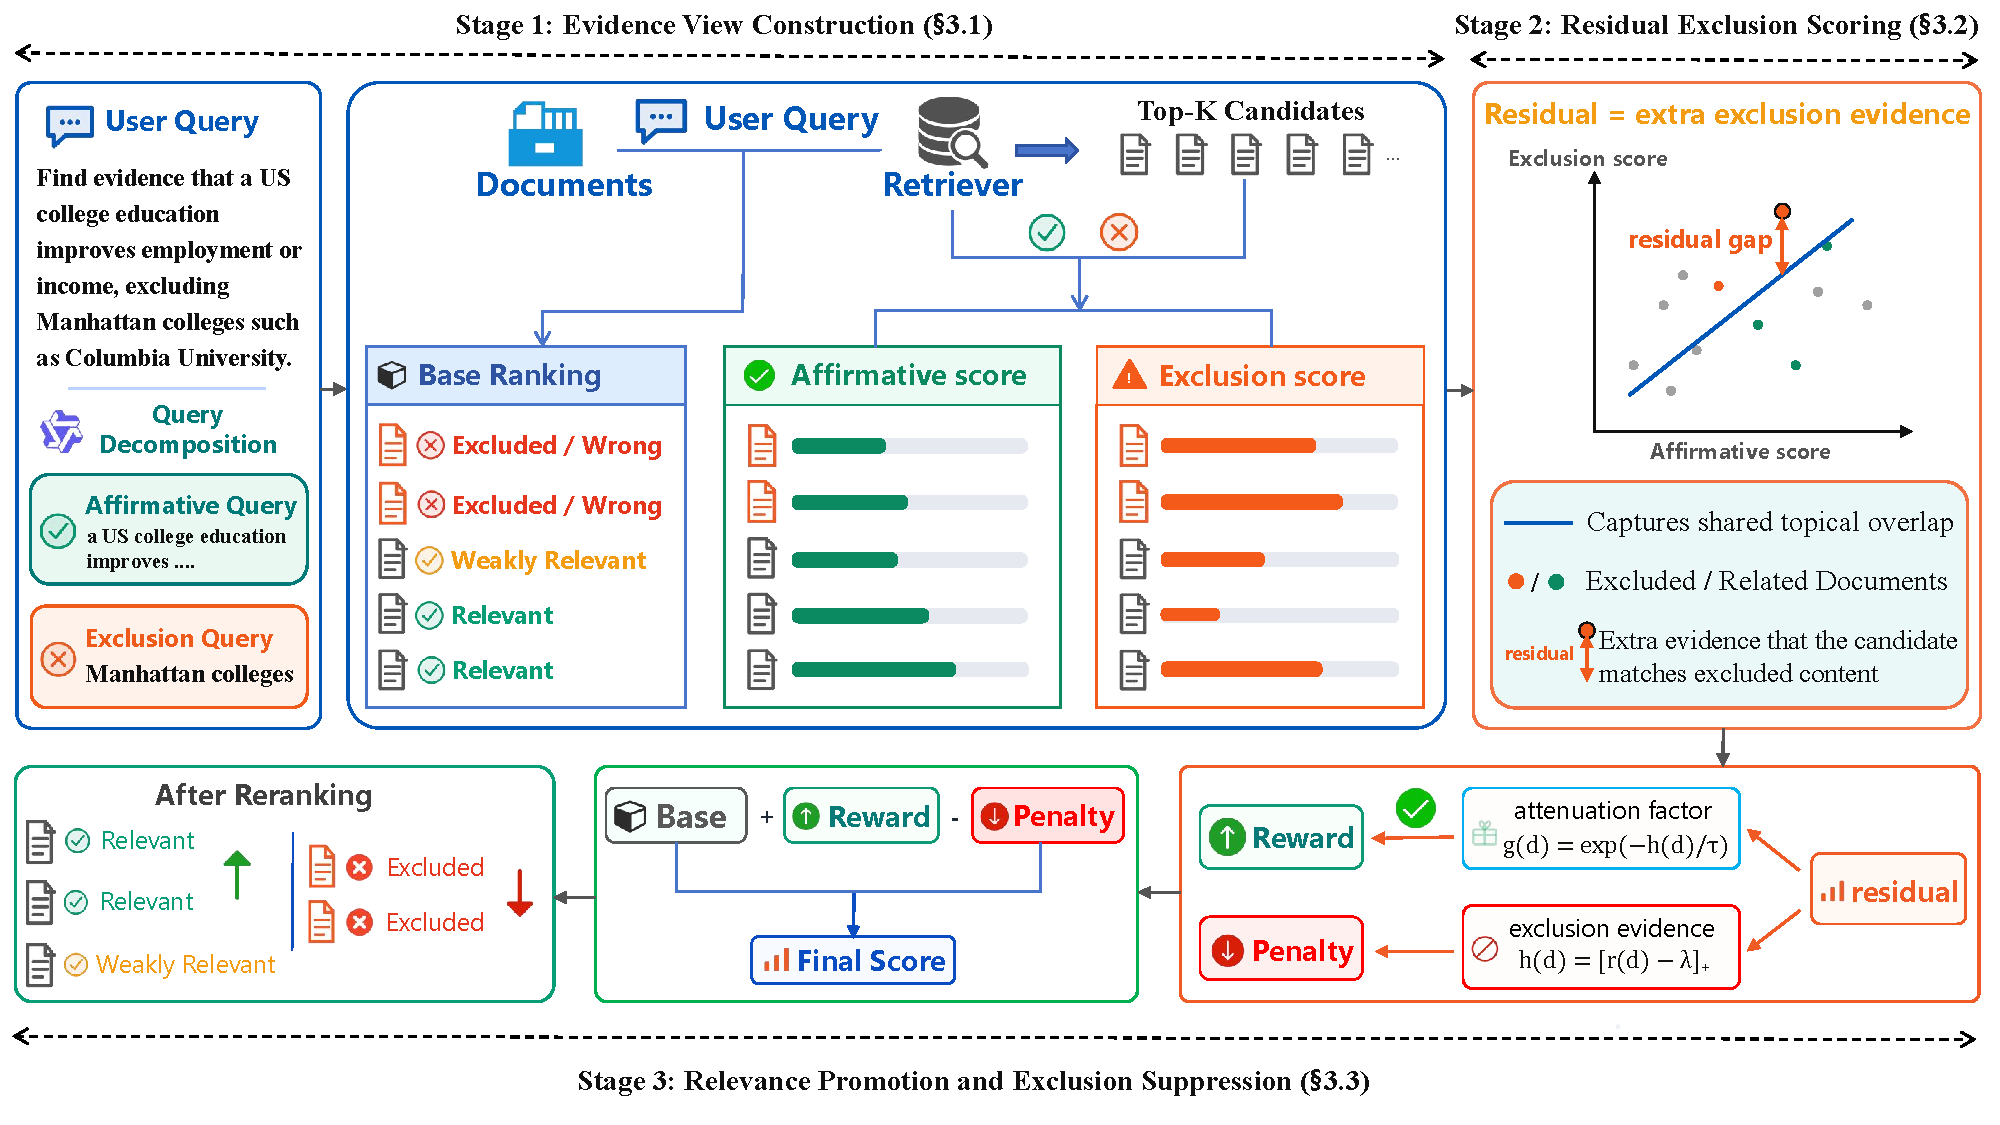
\includegraphics[width=\textwidth]{Figures/framework.pdf}
\caption{Overview of \method.  Stage 1, Evidence View Construction
(Section~\ref{sec:evidence-views}), constructs full, affirmative, and exclusion
views and retrieves candidates with the full view.  Stage 2, Residual
Exclusion Scoring (Section~\ref{sec:residual-score}), forms a query-local
residual after removing shared score variation over the retrieved documents.  Stage 3,
Relevance Promotion and Exclusion Suppression
(Section~\ref{sec:asymmetric-scoring}), converts this evidence into the final
ranking correction.}
\label{fig:trix-overview}
\end{figure*}

\section{Methodology}
\label{sec:method}

Figure~\ref{fig:trix-overview} presents the three stages of \method.
Section~\ref{sec:evidence-views} constructs full, affirmative, and exclusion
evidence views.  Section~\ref{sec:residual-score} computes a residual score
as a query-local proxy for exclusion evidence beyond topical match.
Section~\ref{sec:asymmetric-scoring} uses this score to promote affirmative
relevance and suppress strong exclusion matches.

\subsection{Evidence View Construction}
\label{sec:evidence-views}

Stage 1 in Figure~\ref{fig:trix-overview} constructs full, affirmative, and
exclusion views while retaining the complete request for initial retrieval.
The base ranking shows why the auxiliary views are needed: two documents about
excluded Manhattan colleges are ranked first because they match both the
desired college-employment topic and the excluded entities named in the
request.  The retriever treats both forms of lexical or embedding similarity
as positive signals without reliably distinguishing their roles in the
instruction.

\method receives a natural-language request $u$ containing the retrieval topic
and its instructions.  The frozen retriever uses the complete request as the
full query $\qbase=u$ and returns the top-$K$ candidate set
$\mathcal C_u$.  An LLM decomposes $u$ once into two auxiliary queries:
$\qpos$ states the content that supports relevance, and $\qneg$ states the
content to exclude.  If the request contains no exclusion, the decomposer
returns $\qneg=\textnormal{[NONE]}$.  The candidate set is always retrieved
with $\qbase$; the auxiliary views are used only for reranking.

Table~\ref{tab:trix-decomposition} illustrates this decomposition using the
running example.  The affirmative view retains the desired content, and the
exclusion view converts the rejected content into a directly scorable
description.

\begin{table}[htbp]
\centering
\small
\setlength{\tabcolsep}{3pt}
\begin{tabular}{p{0.18\linewidth} p{0.73\linewidth}}
\toprule
\textbf{View} & \textbf{Example text} \\
\midrule
$\qbase$ & Find evidence that a US college education improves employment
prospects or income. Exclude documents about colleges in Manhattan, such as
Columbia University. \\
$\qpos$ & Evidence that a US college education improves employment prospects
or income. \\
$\qneg$ & Colleges in Manhattan, such as Columbia University. \\
\bottomrule
\end{tabular}
\caption{Evidence views for the running example in
Figure~\ref{fig:trix-overview}.  The affirmative view states the desired
evidence, while the exclusion view states the content to be excluded.}
\label{tab:trix-decomposition}
\end{table}

The three views serve different roles.  The full query retains the complete
topic, context, and instruction during candidate generation.  The affirmative
view keeps the target topic and positive relevance requirements while removing
the exclusion clause and background information that does not determine
relevance.  The exclusion view states the rejected content as a positive
description, allowing the retriever to score whether a document matches that
content.  In addition to supporting relevance, the affirmative score provides
a reference for the topical component shared with the exclusion score.  All
views use the same frozen scorer.

Let $s(Q,d)$ denote the score assigned to document $d$ under query $Q$.  For
each $d\in\mathcal C_u$, the three channels are
\begin{equation}
\begin{aligned}
 \sbase(d) &= s(\qbase, d), \\
 \spos(d)  &= s(\qpos, d), \\
 \sneg(d)  &= s(\qneg, d).
\end{aligned}
\label{eq:trix-channels}
\end{equation}
For a dense retriever, $s(Q_x,d)=\cos(f_q(Q_x),f_d(d))$ is the embedding
similarity; for BM25, it is the lexical retrieval score.  Dense document
embeddings are computed once and reused across views, while BM25 uses one
fixed index.

\subsection{Residual Exclusion Scoring}
\label{sec:residual-score}

Stage 2 in Figure~\ref{fig:trix-overview} uses the residual as a query-local
proxy for exclusion evidence beyond topical match.  This avoids strongly
penalizing candidates whose exclusion scores are high only because they closely
match the topic.  In the score plot, the fitted line represents the exclusion
score expected from a candidate's affirmative score.  The fifth, relevant
candidate has high scores in both views but lies close to the fitted line,
indicating that its exclusion score is expected from the shared college
background.  The highlighted orange candidate lies farther above the line and
therefore produces a larger positive residual, indicating additional evidence
that it matches the excluded Manhattan colleges.

\method addresses this ambiguity by estimating how much exclusion similarity
is expected from the affirmative score and using the deviation from this
relation as an exclusion proxy.  Because all candidates in $\mathcal C_u$
are retrieved for the same request, the two scores can rise together when both
respond to the shared topic.  An affine fit provides a simple per-request
estimate of this score dependence.  The intercept captures a common offset, and
the slope captures how the exclusion score changes with the affirmative score.
If the two score channels have no systematic relation, the estimated slope is
expected to be near zero.  The fitted value then becomes approximately
constant, so the standardized residual reduces to the normalized exclusion
score up to centering and scaling.

\method first robustly standardizes all three score channels over the retrieved
set $\mathcal C_u$:
\begin{equation}
\begin{aligned}
 z_x(d)&=\frac{S_x(d)-\operatorname{median}_{d'\in\mathcal C_u}S_x(d')}
 {\operatorname{MAD}_{d'\in\mathcal C_u}(S_x(d'))+\epsilon},\\
 &\qquad x\in\{\mathrm{full},\mathrm{pos},\mathrm{neg}\},
\end{aligned}
\label{eq:trix-normalization}
\end{equation}
where $\operatorname{MAD}(S)=\operatorname{median}|S-\operatorname{median}(S)|$
and $\epsilon>0$ prevents division by zero.  This normalization aligns
query-specific offsets and scales while limiting the influence of extreme
scores \cite{rousseeuw1993mad}.  \method then fits the affine relation with
Huber regression:
\begin{equation}
 (\hat a_u,\hat b_u)=\arg\min_{a,b}\sum_{d\in\mathcal C_u}
 \rho_\delta\!\left(z_{\mathrm{neg}}(d)-a-bz_{\mathrm{pos}}(d)\right),
 \label{eq:trix-huber}
\end{equation}
where $\rho_\delta$ is the Huber loss with transition point $\delta$.  The fit
captures the dominant score association, while the Huber loss limits the
influence of large deviations \cite{huber1964robust}.  It provides a
query-specific reference for exclusion similarity.  If
the unnormalized positive-score channel has
$\operatorname{MAD}(S_{\mathrm{pos}})<\epsilon$, we set $\hat b_u=0$ and use
a constant fitted value.
For $e(d)=z_{\mathrm{neg}}(d)-\hat a_u-\hat b_u z_{\mathrm{pos}}(d)$,
we robustly standardize the residual:
\begin{equation}
 r(d)=\frac{e(d)-\operatorname{median}_{d'\in\mathcal C_u}e(d')}
 {\operatorname{MAD}_{d'\in\mathcal C_u}(e(d'))+\epsilon}.
 \label{eq:trix-residual}
\end{equation}
The second standardization makes residual magnitudes comparable across
requests: $r(d)=0$ is the median fitted deviation, and one unit is measured
relative to the within-request residual dispersion.  This common scale allows
the same decision parameters to be used across queries and retrievers.
Positive $r(d)$ indicates more exclusion similarity than predicted by the
document's affirmative score; negative $r(d)$ indicates less.  The residual is
a relative score-space proxy, not a calibrated probability of constraint
violation.  As detailed in the next stage, a residual value above the shared
boundary reduces the affirmative reward and activates an exclusion penalty.
Numerical details are given in
Appendix~\ref{app:implementation}.

\subsection{Relevance Promotion and Exclusion Suppression}
\label{sec:asymmetric-scoring}

Stage 3 in Figure~\ref{fig:trix-overview} uses the residual proxy to control
the final score correction.  Candidates with strong affirmative support and a
small residual retain a positive correction, while candidates with a large
positive residual lose this support and receive a
penalty.  This raises relevant candidates and pushes the two initially
top-ranked but excluded documents downward.  We implement this correction by
first retaining the positive part of the normalized affirmative score:
\begin{equation}
 p(d)=[z_{\mathrm{pos}}(d)]_+.
 \label{eq:trix-positive}
\end{equation}
Because $z_{\mathrm{pos}}(d)$ is median-centered, $p(d)$ rewards only documents
whose affirmative score is above the candidate-set median.  We activate the
exclusion correction beyond a shared boundary $\lambda\geq0$:
\begin{equation}
 h(d)=[r(d)-\lambda]_+,\qquad
 g(d)=\exp\!\left(-\frac{h(d)}{\tau}\right),\quad \tau>0,
 \label{eq:trix-attenuation}
\end{equation}
where $h(d)$ is the positive residual excess above the boundary and
$g(d)\in(0,1]$ is the reward attenuation factor.  Below the boundary,
$h(d)=0$ and $g(d)=1$; above it, $h(d)$ grows linearly while $g(d)$ decreases
smoothly.
The final score is
\begin{equation}
 \sfinal(d)=z_{\mathrm{full}}(d)+p(d)g(d)-h(d).
 \label{eq:trix-final}
\end{equation}
The term $p(d)g(d)$ retains the affirmative reward below the residual boundary
and attenuates it once the boundary is crossed.  The term $-h(d)$ directly
suppresses candidates with a large positive residual, so the correction can
lower a document below its full-query score.  Because the three score
components are derived from robustly standardized scores, we combine them
using fixed unit weights.  These weights remain unchanged across datasets and
retrievers.  For fixed $z_{\mathrm{full}}(d)$ and $p(d)$,
Eq.~\ref{eq:trix-final} is therefore non-increasing in $r(d)$.
When no exclusion view is present, \method sets $h(d)=0$ and $g(d)=1$, reducing
the score to $z_{\mathrm{full}}(d)+p(d)$.

% ============================================================
% 4. EXPERIMENTS
% ============================================================
\section{Experiments}
\label{sec:experiments}

\subsection{Experimental Setup}
\label{sec:evaluation-overview}

\paragraph{Benchmarks and Metrics.}
FollowIR \cite{DBLP:conf/naacl/WellerCMLCDLS25} measures
instruction-following retrieval on Core17, Robust04, and News21.  We report
aggregate retrieval effectiveness (Score) and p-MRR for instruction
sensitivity; positive p-MRR indicates that rank changes follow the relevance
instruction.  NegConstraint
\cite{xu2025logical} and ExcluIR
\cite{DBLP:conf/aaai/ZhangZ0PRRCR25} evaluate exclusion-aware corpus ranking
(MAP and nDCG@10) and desired--excluded pair ordering (MRR and Right Rank),
respectively.  Eight BEIR datasets \cite{beir2021} measure general retrieval
performance using nDCG@10 and MAP@100.

\paragraph{Models and Settings.}
Frozen Qwen3-4B \cite{yang2025qwen3} produces both auxiliary views in one
generation.  All 3{,}858 decompositions are structurally valid; a stratified
manual audit of 90 requests finds that the affirmative view preserves the topic
and positive criteria in every case and the exclusion view covers 67 of 69
applicable exclusions, with two cases judged unclear
(Appendix~\ref{app:decomposition-audit}).  FollowIR uses BM25
\cite{DBLP:journals/ftir/RobertsonZ09} together with the frozen E5-Mistral
\cite{DBLP:conf/acl/WangYHYMW24}, BGE-large
\cite{DBLP:conf/sigir/XiaoLZMLN24}, and RepLLaMA
\cite{DBLP:conf/sigir/MaWYWL24}; NegConstraint and ExcluIR use
BGE-small-en-v1.5, BGE-large-en-v1.5, BGE-M3
\cite{DBLP:conf/sigir/XiaoLZMLN24}, and RepLLaMA.
We rerank 1,000 full-query candidates except on ExcluIR, where the benchmark
protocol requires full-corpus scoring.  Matched variants share candidates,
views, templates, and document representations.  We select
$\lambda{=}0.5$ and $\tau{=}0.1$ once on the training corpus released with
FollowIR using RepLLaMA, then freeze them across all evaluation datasets and
retrievers; no labels from the reported evaluation sets are used.  Detailed
protocols and configurations are provided in
Appendices~\ref{app:exclusion-benchmarks} and \ref{app:implementation}.
We test matched differences using a two-sided paired randomization test with
Holm correction and a significance threshold of $p<0.05$.

\paragraph{Baselines and Controlled Comparisons.}
On FollowIR, FollowIR-7B \cite{DBLP:conf/naacl/WellerCMLCDLS25},
Promptriever \cite{DBLP:conf/iclr/WellerDLPZH25}, and InstEmb
\cite{gao2026instemb} are included as instruction-trained baselines.
We also reproduce HyDE \cite{DBLP:conf/acl/GaoMLC23}, Query2Doc
\cite{DBLP:conf/emnlp/WangYW23}, and ConvSearch-R1
\cite{DBLP:journals/corr/abs-2503-00223} with RepLLaMA.
On the exclusion benchmarks, NS-IR
\cite{xu2025logical}, DEO
\cite{DBLP:journals/corr/abs-2603-09185}, and SEAL
\cite{DBLP:conf/aaai/ZhangZ0PRRCR25} are included as prior methods.  We
reproduce DEO using the same BGE-large top-1,000 candidates, benchmark split,
and evaluation implementation as \method{} on NegConstraint;
published-reference rows are reported separately from the matched
Base/$+\method$ comparisons.

\subsection{Main Results on Instruction-Following Retrieval}
\label{sec:main-results}

Table~\ref{tab:followir-main} reports aggregate FollowIR results.  The lower
block contains matched Base/$+\method$ pairs spanning BM25 and three dense
retriever families; the upper block reports instruction-trained retrievers.
Per-dataset results are reported in
Appendix~\ref{app:followir-breakdown}.

\begin{table}[t]
\centering
\small
\setlength{\tabcolsep}{5pt}
\begin{tabular}{lcc}
\toprule
\textbf{Method} & \textbf{Score $\uparrow$} & \textbf{p-MRR $\uparrow$} \\
\midrule
\multicolumn{3}{l}{\emph{Instruction-trained retrievers}} \\
FollowIR-7B & 24.8 & +12.2 \\
Promptriever & 26.1 & +11.2 \\
InstEmb (Llama-3-8B) & \textbf{28.5} & \textbf{+15.6} \\
\midrule
\multicolumn{3}{l}{\emph{Matched frozen-backbone comparisons}} \\
BM25 & 15.2 & +1.1 \\
\quad $+\method$ & 17.3 & \textbf{+17.5} \\
\addlinespace[2pt]
E5-Mistral & 26.1 & $-$2.7 \\
\quad $+\method$ & 28.0 & +12.1 \\
\addlinespace[2pt]
BGE-large & 19.2 & $-$2.2 \\
\quad $+\method$ & 23.3 & +6.5 \\
\addlinespace[2pt]
RepLLaMA & 23.8 & $-$3.3 \\
\quad $+\method$ & \textbf{28.7} & +12.3 \\
\bottomrule
\end{tabular}
\caption{Aggregate FollowIR results.  Score averages MAP on Core17 and
Robust04 with nDCG on News21.  Each $+\method$ row is matched to the backbone
above it; values are percentages ($\times100$).  Best results within each
comparable block are shown in bold.}
\label{tab:followir-main}
\end{table}

\method improves both retrieval effectiveness and instruction sensitivity for
every frozen backbone, spanning BM25 and three dense retrievers.  Before
reranking, the three dense backbones have negative average p-MRR, indicating
that their rankings often fail to follow the relevance instruction.  \method
makes p-MRR positive while also raising Score; with RepLLaMA, Score increases
from 23.8 to 28.7 and p-MRR from $-3.3$ to $+12.3$; both improvements are
statistically significant ($p<0.05$).
Each Base/$+\method$ pair ranks the same candidates with the same document
representations; \method only corrects their scores.

\paragraph{Comparison with Query Rewriting and Expansion.}
\label{sec:rewrite-comparison}
Table~\ref{tab:followir-full} compares \method{} with representative
inference-time rewriting and expansion methods using RepLLaMA.  Each method
uses its original query-generation and retrieval procedure.  Results for
Core17, Robust04, and News21 are provided in Appendix
Table~\ref{tab:rewrite-breakdown}.

\begin{table}[t]
\centering
\small
\setlength{\tabcolsep}{5pt}
\begin{tabular}{lcc}
\toprule
\textbf{Method} & \textbf{Score $\uparrow$} & \textbf{p-MRR $\uparrow$} \\
\midrule
RepLLaMA & 23.8 & $-$3.3 \\
HyDE & 23.3 & +1.4 \\
Query2Doc & 25.6 & $-$1.1 \\
ConvSearch-R1 & 23.4 & +0.2 \\
\method{} & \textbf{28.7} & \textbf{+12.3} \\
\bottomrule
\end{tabular}
\caption{Aggregate FollowIR comparison with query rewriting and expansion
using RepLLaMA.  Score averages MAP on Core17 and Robust04 with nDCG on
News21; values are percentages ($\times100$).  Best results are shown in
bold.}
\label{tab:followir-full}
\end{table}

\method{} outperforms all compared rewriting and expansion methods on both
aggregate metrics, reaching 28.7 Score and $+12.3$ p-MRR.  Existing rewriting
methods are mainly designed to make the target topic easier to match.  For
example, HyDE generates a hypothetical relevant document, while Query2Doc
expands the query with a generated pseudo-document.  Both add positive topical
context, but neither represents excluded content as evidence that should lower
a document's rank.  Excluded entities can therefore remain strong lexical or
semantic matching signals after rewriting.  \method{} separates
affirmative and exclusion evidence before correcting the ranking scores. 

\subsection{Evaluation on Exclusion-Aware Benchmarks}
\label{sec:exclusion-transfer}

We evaluate \method{} on two benchmarks designed for retrieval with negative
constraints.  NegConstraint \cite{xu2025logical} evaluates compositional
constraints over a ranked corpus, while ExcluIR
\cite{DBLP:conf/aaai/ZhangZ0PRRCR25} compares desired and excluded documents in
pairs.

NegConstraint reranks 1,000 candidates, whereas ExcluIR scores its full corpus;
Appendix~\ref{app:exclusion-benchmarks} provides the evaluation protocol.

\method improves both metrics for every matched backbone on both benchmarks.
RepLLaMA provides the strongest overall results: \method raises its
MAP from 72.8 to 80.0 and nDCG@10 from 79.4 to 84.8 on NegConstraint, while
improving MRR from 75.9 to 87.2 and RR from 62.1 to 89.9 on ExcluIR.
For RepLLaMA, the improvements in both metrics are statistically significant
on each benchmark ($p<0.05$).
Under the matched BGE-large NegConstraint setup, \method reaches 76.6 MAP and
81.8 nDCG@10, exceeding DEO by 3.4 and 3.0 points, respectively.  It also
exceeds the reproduced DEO results and the reported SEAL results on ExcluIR.

\begin{table}[t]
\centering
\small
\setlength{\tabcolsep}{3.2pt}
\begin{tabular}{@{}lcccc@{}}
\toprule
\multirow{2}{*}{\textbf{Backbone / Method}} &
\multicolumn{2}{c}{\textbf{NegConstraint}} &
\multicolumn{2}{c}{\textbf{ExcluIR}} \\
\cmidrule(lr){2-3}\cmidrule(lr){4-5}
& \textbf{MAP $\uparrow$} & \textbf{nDCG@10 $\uparrow$} & \textbf{MRR $\uparrow$} & \textbf{RR $\uparrow$} \\
\midrule
\multicolumn{5}{l}{\emph{External and reproduced baselines}} \\
NS-IR (GPT-4o) & 53.3 & 56.5 & --- & --- \\
DEO (BGE-large) & \textbf{73.2} & \textbf{78.8} & 74.1 & \textbf{79.3} \\
SEAL (trained) & --- & --- & \textbf{78.4} & 78.0 \\
\midrule
\multicolumn{5}{l}{\emph{Matched frozen-backbone comparisons}} \\
BGE-small & 68.4 & 75.2 &
75.0 & 60.1 \\
\quad $+\method$ & 76.9 & 82.3 &
77.1 & 81.3 \\
\addlinespace[2pt]
BGE-large & 63.8 & 71.9 &
73.4 & 56.0 \\
\quad $+\method$ & 76.6 & 81.8 &
78.2 & 82.2 \\
\addlinespace[2pt]
BGE-M3 & 64.3 & 74.1 &
78.9 & 67.0 \\
\quad $+\method$ & 74.7 & 81.1 &
79.7 & 83.7 \\
\addlinespace[2pt]
RepLLaMA & 72.8 & 79.4 &
75.9 & 62.1 \\
\quad $+\method$ & \textbf{80.0} & \textbf{84.8} &
\textbf{87.2} & \textbf{89.9} \\
\bottomrule
\end{tabular}
\caption{Results on NegConstraint and ExcluIR.  NegConstraint uses top-1,000
candidates, whereas ExcluIR scores its full 90,406-document corpus.  Each
$+\method$ row uses the same candidate pool and document representations as
its base.  DEO results are our BGE-large reproductions; its NegConstraint run
uses the same candidate and evaluation setup as the BGE-large \method{}
experiment.  Values are percentages ($\times100$).  Best results within each
comparable block are shown in bold.}
\label{tab:exclusion-transfer}
\end{table}

\subsection{General Retrieval Performance}
\label{sec:beir-preservation}

Table~\ref{tab:beir-main} reports average results on eight BEIR datasets; the
per-dataset breakdown is in Appendix~\ref{app:beir}.

\begin{table}[t]
\centering
\small
\setlength{\tabcolsep}{6pt}
\begin{tabular}{lcc}
\toprule
\textbf{Method} & \textbf{Avg.\ nDCG@10 $\uparrow$} & \textbf{Avg.\ MAP@100 $\uparrow$} \\
\midrule
BGE-large & 60.02 & 44.97 \\
\quad $+\method$ & 60.23 & 44.92 \\
\bottomrule
\end{tabular}
\caption{General retrieval performance on eight BEIR datasets with BGE-large.
\method{} maintains average retrieval effectiveness, with changes of $+0.21$
nDCG@10 and $-0.05$ MAP@100; values are percentages ($\times100$).}
\label{tab:beir-main}
\end{table}

Average nDCG@10 changes from 60.02 to 60.23 and MAP@100 from 44.97 to 44.92.
These small aggregate changes show that \method{} improves instruction sensitive retrieval while maintaining strong general retrieval performance.

\subsection{Ablation Study}
\label{sec:ablation-study}

Table~\ref{tab:ablation-residual} organizes the ablation around three design
steps: evidence view construction, residual exclusion scoring, and final score
correction.  Here $p$, $r$, $h$, and $g$ denote the positive score, residual
exclusion score, thresholded exclusion penalty, and reward attenuation factor
defined in Section~\ref{sec:method}.  All variants use the same
candidates, generated views, frozen encoder, templates, embeddings, and
hyperparameters.

\begin{table}[t]
\centering
\small
\setlength{\tabcolsep}{2pt}
\begin{tabular}{lccc}
\toprule
\textbf{Variant} & \textbf{Decision score} & \textbf{Score} & \textbf{p-MRR} \\
\midrule
\multicolumn{4}{l}{\emph{Evidence construction}} \\
Full-query baseline & $z_{\mathrm{full}}$ & 23.8 & $-$3.3 \\
Positive-view scoring & $z_{\mathrm{full}}+p$ & 25.5 & $-$0.7 \\
Exclusion-view subtraction & $z_{\mathrm{full}}-z_{\mathrm{neg}}$ & 25.8 & +7.6 \\
\midrule
\multicolumn{4}{l}{\emph{Exclusion-signal construction}} \\
Raw exclusion subtraction & $z_{\mathrm{full}}+p-z_{\mathrm{neg}}$ & 24.0 & +14.9 \\
Residual exclusion subtraction & $z_{\mathrm{full}}+p-r$ & 26.6 & +12.7 \\
\midrule
\multicolumn{4}{l}{\emph{\method score composition}} \\
\method w/o reward attenuation & $z_{\mathrm{full}}+p-h$ & 27.1 & +10.8 \\
\method w/o exclusion penalty & $z_{\mathrm{full}}+pg$ & 26.2 & +8.9 \\
Full \method & $z_{\mathrm{full}}+pg-h$ & \textbf{28.7} & \textbf{+12.3} \\
\bottomrule
\end{tabular}
\caption{Controlled mechanism ablation on FollowIR.  The three blocks isolate
evidence construction, exclusion-signal construction, and the two operations
in \method score composition.  Score averages MAP on Core17 and Robust04 with
nDCG on News21; all values are percentages ($\times100$).  Results for the
full system are shown in bold.}
\label{tab:ablation-residual}
\end{table}

\paragraph{Evidence Views.}
The focused positive view raises Score from 23.8 to 25.5 and p-MRR from
$-3.3$ to $-0.7$, confirming that it contributes evidence beyond the full
instruction.  The exclusion view also contributes independently: subtracting
its score raises Score to 25.8 and p-MRR to $+7.6$.  The two views therefore
provide complementary signals for relevance promotion and exclusion
suppression.

\paragraph{Residual Exclusion Evidence.}
Raw subtraction aggressively lowers documents with high exclusion scores,
including both exclusion matches and relevant documents whose scores are high
because of shared topic content.  The resulting rank changes produce a higher
p-MRR of $+14.9$, but the collateral suppression of relevant documents lowers
Score to 24.0.  Measuring exclusion evidence relative to the affirmative score
makes the correction more selective: p-MRR decreases to $+12.7$, while Score
rises to 26.6.  The residual therefore reduces broad rank disruption and
preserves more relevant documents.

\paragraph{Score Correction.}
Full \method
improves over the variant without reward attenuation by 1.6 Score and 1.5
p-MRR points, showing that strong residual evidence should also reduce the
positive contribution.  Adding the explicit penalty to the attenuation-only
variant yields gains of 2.5 Score and 3.4 p-MRR points.  Together, the two
comparisons support the asymmetric combination of attenuating affirmative
support and directly suppressing strong exclusion matches.

\subsection{Mechanism Analysis}
\label{sec:mechanism-analysis}

\paragraph{Residual Signal.}
Figure~\ref{fig:residual-mechanism} illustrates how residualization changes
the meaning of the exclusion score.  In the left panel, $z_{\mathrm{neg}}$
increases strongly with $z_{\mathrm{pos}}$ (Pearson $r=0.93$), showing that
the two views share substantial topical information.  The dashed Huber fit
estimates the exclusion score expected from this association.  Many blue
relevant documents have relatively high raw exclusion scores, yet lie below
the fitted relation; directly subtracting $z_{\mathrm{neg}}$ would therefore
penalize them for similarity already explained by their affirmative scores.

\begin{figure}[t]
\centering
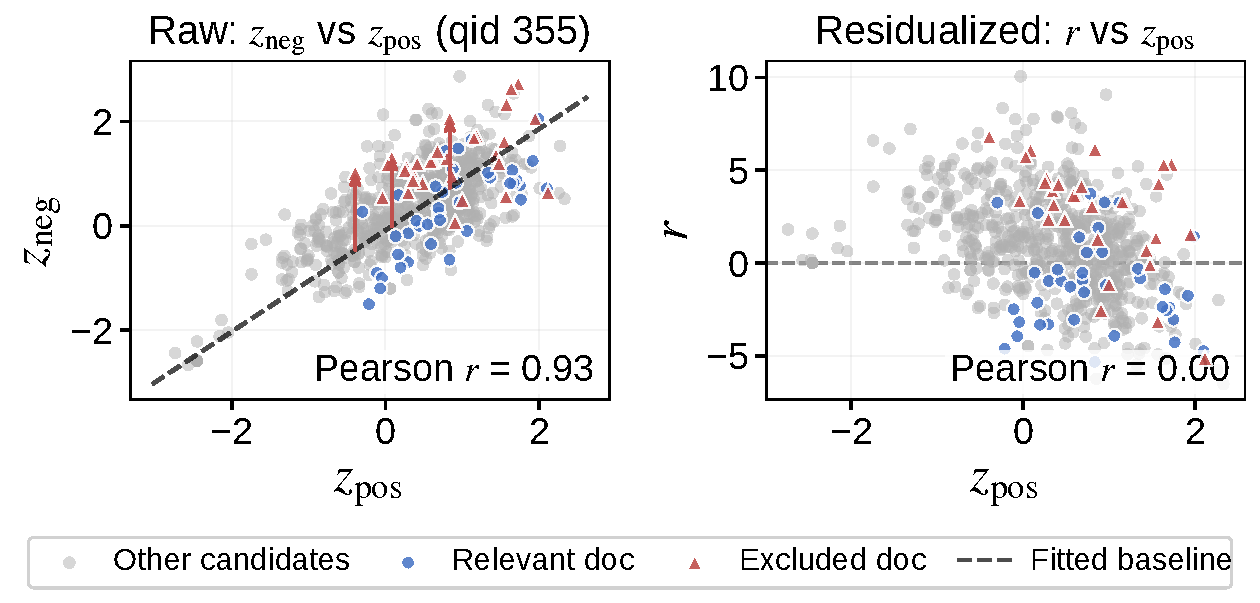
\includegraphics[width=0.94\linewidth]{Figures/figure2_adjusted_aaai27_fontlarge_v7.pdf}
\caption{Residualization for an illustrative query.  Blue circles denote
relevant documents, red triangles denote excluded documents, and gray circles
denote other candidates.  Left: the dashed Huber fit captures the strong
association between affirmative and exclusion scores.  Right: standardized
deviations from the fit; the dashed horizontal line marks $r=0$.}
\label{fig:residual-mechanism}
\end{figure}

The right panel shows the standardized residual after removing the fitted
component.  Its correlation with $z_{\mathrm{pos}}$ falls to $0.00$, indicating
that the shared score trend has been removed.  Many blue relevant documents
now fall below $r=0$ and therefore remain below the correction boundary, preserving their affirmative reward and avoiding an exclusion
penalty.  Most red excluded documents retain positive residuals because their
exclusion similarity exceeds the level predicted by their affirmative score.
This more selective correction matches Table~\ref{tab:ablation-residual}:
compared with raw subtraction, residualization reduces p-MRR from $+14.9$ to
$+12.7$ as the rank changes become less aggressive, while increasing Score
from 24.0 to 26.6 by preserving more relevant documents.

\paragraph{Ranking Behavior.}
Figure~\ref{fig:reward-penalty-effect} visualizes the document-level rank
changes produced by \method{}.

\begin{figure}[t]
\centering
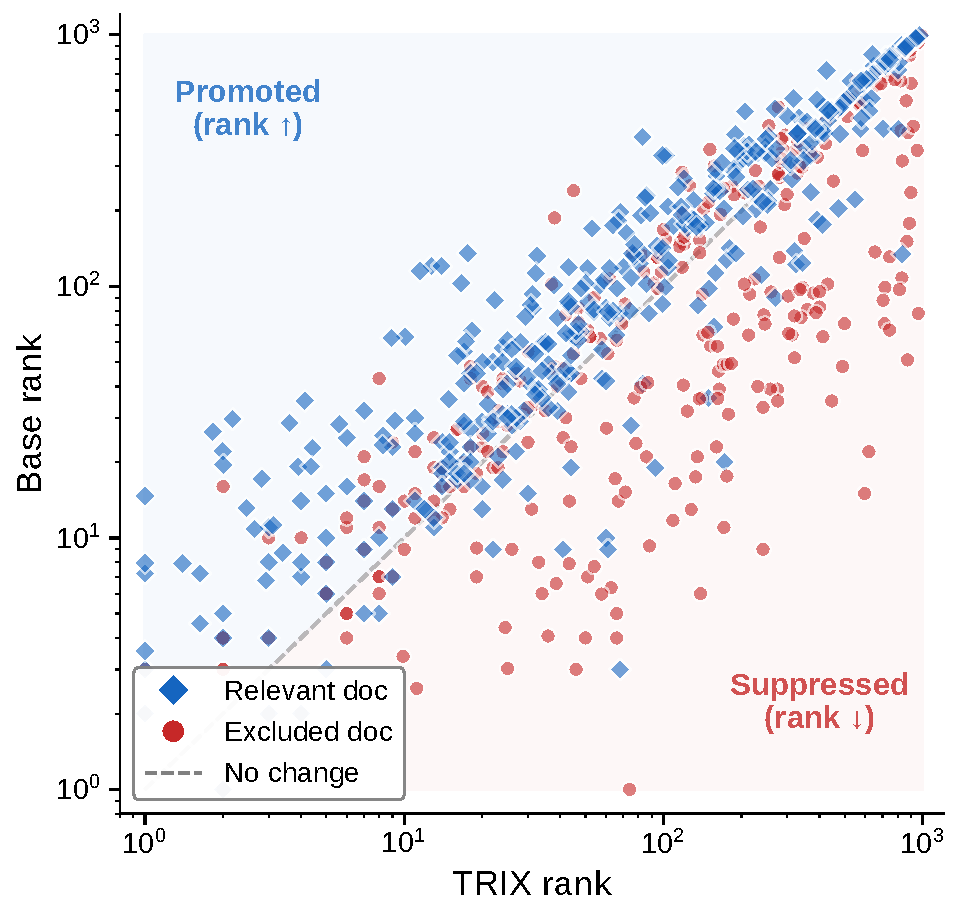
\includegraphics[width=0.85\linewidth]{Figures/dual_rank_scatter_followir_repllama_v8_aaai27_fontfix_v2.pdf}
\caption{Rank changes produced by \method{} on FollowIR exclusion queries.
The vertical axis gives the initial rank from the frozen retriever, and the
horizontal axis gives the rank after \method{} adds the affirmative reward and
subtracts the exclusion penalty.  Points above the diagonal are promoted,
points below it are suppressed, and points on the diagonal are unchanged.
Blue diamonds denote relevant documents, while red circles denote
documents that violate the exclusion constraint.}
\label{fig:reward-penalty-effect}
\end{figure}

Because smaller rank values are better, a point above the diagonal has a
better \method{} rank than its base rank, whereas a point below the diagonal
has been pushed downward.  The blue diamonds concentrate above the diagonal,
showing that most relevant documents receive a net promotion from the
affirmative reward. The red circles concentrate below the diagonal, showing
that documents violating the exclusion are generally suppressed by the
residual-controlled penalty. Points close to the diagonal receive
smaller corrections and retain similar ranks.  This separation
shows that \method{} directs its two scoring operations toward the intended
documents: relevance promotion primarily benefits relevant documents, and
exclusion suppression primarily lowers documents that violate the constraint.

% ============================================================
% 5. CONCLUSION AND LIMITATIONS
% ============================================================
\section{Conclusion and Limitations}
\label{sec:conclusion}

This paper presented \method{}, a training-free score correction method for
frozen retrievers.  Its evidence views improve relevance scoring, while
residual exclusion scoring reduces penalties caused by shared topic
information.  Across sparse and dense retrievers, the resulting correction
improves instruction-sensitive ranking while maintaining general retrieval
performance.

\method requires useful decomposed views and adequate initial candidate
coverage; as a reranker, it cannot recover documents absent from the retrieved
set.  The residual may also be less informative when the exclusion view
provides little evidence in that set.  Stronger decomposition and candidate
generation are natural directions for future work.

% ============================================================
% REFERENCES
% ============================================================
{\small
\bibliography{references}
}

% ============================================================
% APPENDIX
% ============================================================
\clearpage
\appendix

\section{Full FollowIR Results}
\label{app:followir-breakdown}

Table~\ref{tab:followir-breakdown} provides the per-dataset results
underlying the aggregate comparison in Table~\ref{tab:followir-main}.
Results for instruction-trained methods are taken from their source papers
\cite{DBLP:conf/naacl/WellerCMLCDLS25,DBLP:conf/iclr/WellerDLPZH25,
gao2026instemb}.

\begin{table}[htbp]
\centering
\small
\setlength{\tabcolsep}{3.2pt}
\textit{(a) Retrieval effectiveness $\uparrow$}\par\smallskip
\begin{tabular}{lcccc}
\toprule
\textbf{Method} & \textbf{Core17} & \textbf{Robust04} &
\textbf{News21} & \textbf{Score} \\
\midrule
\multicolumn{5}{l}{\emph{Instruction-trained retrievers}} \\
FollowIR-7B & 20.0 & 24.8 & 29.6 & 24.8 \\
Promptriever & 21.6 & 28.3 & 28.5 & 26.1 \\
InstEmb (Llama-3-8B) & 24.0 & 29.2 & 32.3 & 28.5 \\
\midrule
\multicolumn{5}{l}{\emph{Matched frozen-backbone comparisons}} \\
BM25 & 10.8 & 13.8 & 21.0 & 15.2 \\
\quad $+\method$ & 13.2 & 14.0 & 24.8 & 17.3 \\
E5-Mistral & 20.4 & 27.9 & 30.1 & 26.1 \\
\quad $+\method$ & 24.4 & 26.7 & 32.8 & 28.0 \\
BGE-large & 16.8 & 19.4 & 21.4 & 19.2 \\
\quad $+\method$ & 22.1 & 21.9 & 26.0 & 23.3 \\
RepLLaMA & 23.2 & 25.7 & 22.5 & 23.8 \\
\quad $+\method$ & 25.9 & 28.2 & 32.1 & 28.7 \\
\bottomrule
\end{tabular}

\smallskip
\textit{(b) Instruction sensitivity (p-MRR $\uparrow$)}\par\smallskip
\begin{tabular}{lcccc}
\toprule
\textbf{Method} & \textbf{Core17} & \textbf{Robust04} &
\textbf{News21} & \textbf{Average} \\
\midrule
\multicolumn{5}{l}{\emph{Instruction-trained retrievers}} \\
FollowIR-7B & +16.5 & +13.7 & +6.3 & +12.2 \\
Promptriever & +15.4 & +11.7 & +6.4 & +11.2 \\
InstEmb (Llama-3-8B) & +22.4 & +19.1 & +5.4 & +15.6 \\
\midrule
\multicolumn{5}{l}{\emph{Matched frozen-backbone comparisons}} \\
BM25 & +3.7 & $-$0.5 & 0.0 & +1.1 \\
\quad $+\method$ & +18.4 & +13.8 & +20.3 & +17.5 \\
E5-Mistral & $-$0.3 & $-$6.9 & $-$0.9 & $-$2.7 \\
\quad $+\method$ & +5.7 & +19.6 & +11.1 & +12.1 \\
BGE-large & $-$2.0 & $-$5.2 & +0.5 & $-$2.2 \\
\quad $+\method$ & +4.3 & +9.0 & +6.3 & +6.5 \\
RepLLaMA & +1.1 & $-$9.1 & $-$1.8 & $-$3.3 \\
\quad $+\method$ & +16.2 & +14.1 & +6.7 & +12.3 \\
\bottomrule
\end{tabular}
\caption{Per-dataset FollowIR results.  The two panels report retrieval
effectiveness and p-MRR for the same systems; values are percentages
($\times100$).}
\label{tab:followir-breakdown}
\end{table}

\begin{table}[t]
\centering
\small
\setlength{\tabcolsep}{3.2pt}
\textit{(a) Retrieval effectiveness $\uparrow$}\par\smallskip
\begin{tabular}{lcccc}
\toprule
\textbf{Method} & \textbf{Core17} & \textbf{Robust04} &
\textbf{News21} & \textbf{Score} \\
\midrule
RepLLaMA & 23.2 & 25.7 & 22.5 & 23.8 \\
HyDE & 23.6 & 24.9 & 21.4 & 23.3 \\
Query2Doc & 25.9 & 26.1 & 24.9 & 25.6 \\
ConvSearch-R1 & 22.3 & 25.9 & 22.0 & 23.4 \\
\method{} & 25.9 & 28.2 & 32.1 & 28.7 \\
\bottomrule
\end{tabular}

\smallskip
\textit{(b) Instruction sensitivity (p-MRR $\uparrow$)}\par\smallskip
\begin{tabular}{lcccc}
\toprule
\textbf{Method} & \textbf{Core17} & \textbf{Robust04} &
\textbf{News21} & \textbf{Average} \\
\midrule
RepLLaMA & +1.1 & $-$9.1 & $-$1.8 & $-$3.3 \\
HyDE & +6.5 & $-$2.9 & +0.7 & +1.4 \\
Query2Doc & +8.0 & $-$7.5 & $-$3.8 & $-$1.1 \\
ConvSearch-R1 & +3.0 & $-$2.5 & +0.2 & +0.2 \\
\method{} & +16.2 & +14.1 & +6.7 & +12.3 \\
\bottomrule
\end{tabular}
\caption{Per-dataset FollowIR comparison with query rewriting and
expansion using RepLLaMA.  The two panels report retrieval effectiveness and
p-MRR; values are percentages ($\times100$).}
\label{tab:rewrite-breakdown}
\end{table}

\section{Additional Ablations and Sensitivity}
\label{app:additional-ablations}

The main text isolates the positive view, residual exclusion signal, reward
attenuation, and explicit penalty.  The following results compare alternative
residual estimators and examine sensitivity to the shared configuration.

\subsection{Estimator and Normalization Choices}

Table~\ref{tab:diagnostic-ablation} compares the robust estimator,
normalization, and residual construction used to obtain $r$.

\begin{table}[t]
\centering
\small
\setlength{\tabcolsep}{2.2pt}
\begin{tabular}{p{0.92in}p{1.30in}cc}
\toprule
\textbf{Variant} & \textbf{Modification} & \textbf{Score} & \textbf{p-MRR} \\
\midrule
Full \method{} & None & 28.7 & $+$12.3 \\
\method{} w/ OLS & Replace Huber regression & 26.9 & $+$10.6 \\
\method{} w/ mean/std scaling & Replace median/MAD scaling & 26.8 & $+$8.5 \\
\method{} w/o residual centering & Omit residual recentering & 27.1 & $+$10.8 \\
\bottomrule
\end{tabular}
\caption{Secondary \method design choices on FollowIR.  Each row changes one
estimation or normalization choice while retaining the controlled candidate
set and three evidence views.}
\label{tab:diagnostic-ablation}
\end{table}

\begin{table}[t]
\centering
\small
\setlength{\tabcolsep}{3pt}
\begin{tabular}{llcc}
\toprule
\textbf{Analysis} & \textbf{Setting} & \textbf{Score} &
\textbf{p-MRR} \\
\midrule
Threshold & $\lambda=0.5$ (default) & 28.7 & $+$12.3 \\
& $\lambda=1.0$ & 28.3 & $+$11.8 \\
& $\lambda=1.5$ & 28.1 & $+$9.2 \\
& $\lambda=2.0$ & 27.8 & $+$7.5 \\
\addlinespace[2pt]
Temperature & $\tau=0.1$ (default) & 28.7 & $+$12.3 \\
& $\tau=0.2$ & 28.2 & $+$11.9 \\
& $\tau=0.5$ & 27.8 & $+$10.4 \\
& $\tau=1.0$ & 27.1 & $+$8.7 \\
\addlinespace[2pt]
Candidate depth & $K=10$ & 26.3 & $+$16.1 \\
& $K=50$ & 27.2 & $+$18.8 \\
& $K=100$ & 27.9 & $+$19.5 \\
& $K=200$ & 27.3 & $+$19.8 \\
& $K=1000$ (default) & 28.7 & $+$12.3 \\
\addlinespace[2pt]
Query decomposition & Qwen3-4B & \multicolumn{2}{c}{$2.81\mathbin{\pm}1.20$\,s/q} \\
Post-scoring correction & Cached scores & \multicolumn{2}{c}{$0.4$\,ms/q} \\
\bottomrule
\end{tabular}
\caption{Sensitivity and efficiency with RepLLaMA on FollowIR.  Each
sensitivity block varies one factor while retaining the other defaults
($K{=}1000$, $\lambda{=}0.5$, and $\tau{=}0.1$).  Candidate depth $K$ jointly
specifies the number of $\qbase$ candidates retrieved, used for normalization
and Huber fitting, and reranked before metric computation.  Score and p-MRR are
averaged over the three FollowIR datasets.  Decomposition latency is measured
across all FollowIR queries using Qwen3-4B on a single NVIDIA GeForce RTX 3090
GPU with temperature $0.1$; we report mean $\pm$ standard deviation.  The
$0.4$ ms measurement covers score normalization, Huber fitting, and final
reranking after retrieval scores are available.}
\label{tab:sensitivity-efficiency}
\end{table}

Table~\ref{tab:sensitivity-efficiency} varies one factor at a time around the
main RepLLaMA configuration.  The $K=1000$ row reproduces the main FollowIR
result (28.7 Score and $+12.3$ p-MRR), resolving the candidate-depth setting
used by Tables~\ref{tab:followir-main} and~\ref{tab:followir-full}.  All tested
depths improve over the RepLLaMA base result of 23.8 Score and $-3.3$ p-MRR.
From $K=10$ to $K=200$, p-MRR increases steadily from $+16.1$ to $+19.8$,
while Score rises from 26.3 to 27.9 at $K=100$ before decreasing to 27.3 at
$K=200$.  Expanding the depth to the default $K=1000$ yields the highest Score
of 28.7 but lowers p-MRR to $+12.3$.  The updated results therefore show a
depth-dependent trade-off: shallower candidate sets produce larger measured
instruction-sensitive rank changes, whereas the full depth provides the best
aggregate retrieval effectiveness.  Because the same $K$ determines retrieval
coverage, the pool used for robust normalization and Huber fitting, and the
documents reranked before evaluation, this analysis measures their joint
effect.  Separating candidate coverage from score-estimation effects would
require holding retrieval depth fixed while varying only the estimation pool.
In the one-factor parameter sweeps, increasing either $\lambda$ or $\tau$
reduces both reported metrics relative to the tested defaults.

Instruction decomposition averages $2.81$ seconds per query (standard
deviation $1.20$, range $1.51$--$6.80$ seconds), corresponding to a throughput
of $0.36$ decomposition queries per second.  After the three retrieval-score
channels are available, score normalization, Huber fitting, and final
reranking take $0.4$ ms per query.  This post-scoring measurement excludes
query decomposition, query encoding, and candidate retrieval, and therefore is
not an end-to-end latency measurement.  Among the reported online components,
latency is dominated by the one-time query decomposition.  \method requires no
retriever training, document re-encoding, or candidate-level LLM inference;
its additional LLM cost is one query-level decomposition.

\section{Additional Exclusion-Benchmark Results}
\label{app:exclusion-benchmarks}

Table~\ref{tab:exclusion-transfer} (main text,
Section~\ref{sec:exclusion-transfer}) reports the complete \method results
across NegConstraint and ExcluIR.  Table~\ref{tab:exclusion-ablation} examines
whether its performance depends on using the per-query regression residual
instead of raw exclusion similarity.  The same matched comparison is applied
to both benchmarks.  Within each benchmark, all rows use the same frozen
retriever, candidate pool, decomposition, query templates, document embeddings,
and shared $\lambda,\tau$.  The pool contains the top 1,000 candidates for
NegConstraint and the complete 90,406-document corpus for ExcluIR.  The raw
and residual correction rows differ only in the exclusion signal supplied to
the same \method scoring function.

\paragraph{ExcluIR Evaluation Protocol.}
For an ExcluIR request $u$, let
$\operatorname{rank}_u(d)\in\{1,\ldots,90{,}406\}$ be the one-based rank of
document $d$ after reranking the full corpus.  For an annotated desired
document $d^+$, its top-10 reciprocal-rank contribution is
$1/\operatorname{rank}_u(d^+)$ when $\operatorname{rank}_u(d^+)\leq10$ and
zero otherwise; MRR averages this quantity over the evaluation instances.
For each annotated desired--excluded pair $(d^+,d^-)$, Right Rank is one when
$\operatorname{rank}_u(d^+)<\operatorname{rank}_u(d^-)$ and zero otherwise;
RR is its mean over all pairs.  Equal ranks contribute zero.  Full-corpus
scoring guarantees that neither pair member is missing from the evaluated
ranking.

\paragraph{Result Provenance.}
We reproduce DEO with BGE-large on both benchmarks.  For the controlled
NegConstraint comparison, DEO and \method{} start from the same BGE-large
top-1,000 candidate lists and use the same benchmark split and evaluation
implementation; each method retains its own query construction and scoring
rule.  The ExcluIR values follow the full-corpus protocol above.  The SEAL
ExcluIR values are taken from its source paper.  The matched
Base/$+\method$ blocks isolate \method's score correction, while the controlled
DEO comparison evaluates it against another training-free method under the
same NegConstraint setup.

\begin{table}[t]
\centering
\small
\setlength{\tabcolsep}{3.2pt}
\begin{tabular}{p{1.18in}cccc}
\toprule
\multirow{2}{*}{\textbf{Variant}} &
\multicolumn{2}{c}{\textbf{NegConstraint}} &
\multicolumn{2}{c}{\textbf{ExcluIR}} \\
\cmidrule(lr){2-3}\cmidrule(lr){4-5}
& \textbf{MAP} & \textbf{nDCG@10} & \textbf{MRR} & \textbf{RR} \\
\midrule
Full-query baseline & 63.8 & 71.9 & 73.4 & 56.0 \\
\method{} w/ positive view only & 76.0 & 81.8 & 75.0 & 58.0 \\
\method{} w/ raw exclusion score & 76.6 & 81.8 & 76.0 & 60.0 \\
Full \method{} & 76.6 & 81.8 & 78.2 & 82.2 \\
\bottomrule
\end{tabular}
\caption{Matched exclusion-signal ablation across exclusion benchmarks with
BGE-large-en-v1.5.  Within each benchmark, all variants use the same candidate
pool, generated views, document representations, and scoring hyperparameters.}
\label{tab:exclusion-ablation}
\end{table}

The two benchmarks show different contributions from the exclusion signal.
On NegConstraint, the positive view accounts for most of the gain over the
full-query baseline: it raises MAP from 63.8 to 76.0 and nDCG@10 from 71.9 to
81.8.  Raw exclusion scoring adds 0.6 MAP points and no nDCG@10 gain, while
replacing it with the residual leaves both reported metrics unchanged at 76.6
and 81.8.  On ExcluIR, the residual correction improves over raw exclusion
scoring from 76.0 to 78.2 MRR and from 60.0 to 82.2 RR.  Thus, in this matched
comparison, residualization contributes most clearly to the desired--excluded
pair ordering measured by ExcluIR, whereas the NegConstraint improvement is
driven primarily by the positive view.

\section{Qualitative Analysis}
\label{app:qualitative}

The qualitative analysis draws one example from successful cases and one from
unsuccessful cases on FollowIR Core17 with RepLLaMA.  Each example reports the
benchmark, query ID, complete request, decomposed views, candidate scores, and
ranking change.  The two examples illustrate how the scoring mechanism behaves
under successful and unsuccessful outcomes.  We define the failure pool as
queries for which the final top 10 contains no gold-relevant document and
MRR@10 remains zero.

\begin{table*}[t]
\centering
\small
\setlength{\tabcolsep}{4pt}
\renewcommand{\arraystretch}{1.05}
\begin{tabular}{p{0.10\textwidth}p{0.26\textwidth}p{0.25\textwidth}p{0.27\textwidth}}
\toprule
\textbf{Outcome} & \textbf{Request and views} & \textbf{Candidate evidence} &
\textbf{Ranking effect and interpretation} \\
\midrule
Success &
  Benchmark: FollowIR (Core17), QID 355
  \newline Query: ``Identify documents discussing the development and application of space-borne ocean remote sensing''
  \newline Exclusion: land-bound sciences, agriculture, forestry, marketing, temperature
  \newline Views: $\qbase$ (full query), $\qpos$ (ocean remote sensing in oceanography, seabed prospecting, marine sciences), $\qneg$ (land-bound sciences, agriculture, forestry, marketing, temperature) &
  The original top-1 document scores high on both $s_{\text{pos}}$ and
  $s_{\text{neg}}$ because it contains agriculture and forestry content.
  Residual $r$ remains high after accounting for the shared score variation.
  \newline After \method, an ocean-only document becomes the new top-1, while
  the original land-bound top-1 document drops to rank 580. &
  Land-bound/agriculture documents drop from top-10 to rank $>500$.
  \newline Ocean remote-sensing documents rise to top-5.
  \newline \textbf{Interpretation:} \method{} uses the high residual to suppress the excluded content in this candidate set. \\

Failure &
  Benchmark: FollowIR (Core17), QID 416
  \newline Query: ``What is the ongoing status of The Three Gorges Project?''
  \newline Inclusion: completion date, total cost, or electrical output
  \newline Exclusion: social, political, or ecological impacts and displacement
  \newline Views: $\qbase$ (full request), $\qpos$ (project status through
  completion, cost, and electrical output), $\qneg$ (social, political, and
  ecological impacts; displacement) &
  The final top-5 documents mix requested project facts with explicitly
  excluded impacts.  Under the instruction, all five have FollowIR
  gold relevance 0 and belong to the benchmark's label-difference set.  Their
  residuals range from $-5.10$ to $-2.22$, below $\lambda=0.5$, so $h=0$ and
  $g=1$ for each document; the positive-view reward is retained without an
  exclusion penalty. &
  The original top-1 document remains at rank 1.  The first gold-relevant
  document rises from rank 23 to 13, but none reaches the top 10, and MRR@10
  remains 0.
  \newline \textbf{Interpretation:} Their high positive-view scores raise the
  fitted negative-score expectation, whereas their observed negative-view
  scores remain below that expectation.  The resulting negative residuals
  expose a limitation of relative residual scoring: it can miss hard-constraint
  violations when the excluded content does not produce negative similarity
  beyond that expected from the shared topic. \\
\bottomrule
\end{tabular}
\caption{One successful and one unsuccessful \method{} example drawn from
FollowIR Core17 with RepLLaMA.  Each example reports the operational views,
score-space evidence, and ranking change under the complete scoring rule.}
\label{tab:qualitative-cases}
\end{table*}

\section{Decomposition and Reproducibility Details}
\label{app:implementation}

The instruction decomposer is the frozen Qwen3-4B model
\cite{yang2025qwen3}.  It receives the complete user request and returns
structured affirmative and exclusion content in one generation.  The full
view $\qbase$ is the original request itself, used unchanged for candidate
generation; $\qpos$ retains the topic and affirmative conditions while removing
exclusion content, and $\qneg$ contains the excluded content, or
\textnormal{[NONE]} when no exclusion is present.  We use the fixed prompt with temperature $0.1$, top-$p=0.9$, at most
512 new tokens, and thinking disabled.  Malformed or missing fields are mapped
to the corresponding empty view.  The system prompt is:
{\footnotesize
\begin{verbatim}
You are an expert IR query optimizer
for Dense Vector Models. Decouple
"Original Query" and "Instruction"
into Q_plus and Q_minus.

Q_plus rules: (1) Fluent natural
language phrase, not a keyword list.
(2) Semantic topic only; remove format
noise ("articles", "documents",
"reports"). (3) Remove conversational
connectors ("such as", "including").
(4) Sharp, coherent.

Q_minus rules: (1) Extract only
critical high-level exclusion concepts.
(2) Concise natural phrasing.
(3) If no exclusion, output "[NONE]".

No-negation rule: DENSE RETRIEVERS
IGNORE LOGIC WORDS. NEVER use negation
in Q_minus ("no", "not", "non-",
"without"). Convert negations to
AFFIRMATIVE entities:
  BAD: "not colleges in Manhattan"
  -> GOOD: "colleges in Manhattan,
     such as Columbia University"
Output ONLY exact entities to exclude.

Output JSON:
{
  "Reasoning_Steps": "1. Core topic.
    2. Filter noise. 3. Exclusions
    (negations->affirm).",
  "Q_plus": "Fluent natural language query",
  "Q_minus": "Core exclusions or [NONE]"
}
\end{verbatim}
}
The user prompt template is:
{\footnotesize
\begin{verbatim}
Decouple into Q_plus and Q_minus:
Query: "{query}"
Instruction: "{instruction}"
\end{verbatim}
}

For every backbone, including RepLLaMA, all document representations are
computed once with that retriever's native document template, and all three
query views use its native query template.  Matched Base/$+\method$ variants
reuse the same candidates, templates, and document representations.  The
$K_{\mathrm{retrieve}}=K_{\mathrm{fit}}=K_{\mathrm{rerank}}=1000$ convention
in Section~\ref{sec:evaluation-overview} applies to the reported FollowIR,
NegConstraint, and BEIR results.  ExcluIR uses the complete 90,406-document
corpus as $\mathcal C_u$ for score normalization, Huber fitting, and reranking.

\paragraph{Numerical and Scoring Constants.}
We set the Huber transition point to $\delta=1.35$ in standardized score units.
The constant $\epsilon=10^{-6}$ serves both as the median/MAD denominator
floor and as the low-dispersion threshold: when
$\operatorname{MAD}(S_{\mathrm{pos}})<\epsilon$, the fitted slope is set to
zero.  The regression is fit independently on each candidate set and uses no
relevance labels.  Using RepLLaMA on the FollowIR training corpus, we search
$\lambda\in[0.05,5.0]$ and $\tau\in[0.01,1.0]$ and select
$(\lambda,\tau)=(0.5,0.1)$ based on aggregate Score and p-MRR.  We then freeze
this pair for all evaluation datasets and retrievers, without
per-evaluation-dataset or per-retriever tuning.  Because
$r$ is centered and scaled by its within-query MAD, $\lambda=0.5$ activates
the correction half a residual-MAD unit above the median fitted deviation.
With $\tau=0.1$, each additional $0.1$ active residual unit multiplies the
affirmative reward by $\exp(-1)$.  The full-query score, attenuated affirmative
reward, and residual penalty use unit coefficients; no query-specific scoring
weights are introduced.

\section{Decomposition Quality Audit}
\label{app:decomposition-audit}

We audit the structural and semantic quality of the Qwen3-4B decomposer
output on all three benchmarks used in the paper.

\subsection{Full Structural Validity}
\label{app:structural-validity}

Table~\ref{tab:structural-validity} reports automated checks on every
decomposed record.  All 3{,}858 records parse successfully as valid JSON.
The $\qplus$ field is present and non-trivial in every record.
The $\qminus$ field is present in every record.  The observed [NONE] rates
are $0.5\%$ on NegConstraint and $0.4\%$ on ExcluIR.  On FollowIR,
$38.0\%$ of queries yield $\qminus=\textnormal{[NONE]}$.  These checks establish
field-level validity; the semantic correctness of [NONE] assignments is
assessed separately in Section~\ref{app:semantic-audit}.  No empty-string
$\qplus$ or malformed-field fallback is triggered in any benchmark.

\begin{table}[t]
\centering
\small
\setlength{\tabcolsep}{3pt}
\begin{tabular}{l r c c c c}
\toprule
\textbf{Benchmark} & \textbf{$N$} & \textbf{Parse} &
\textbf{$\qplus$ ok} & \textbf{$\qminus$ ok} & \textbf{[NONE] $\qminus$} \\
\midrule
FollowIR     &   208 & 100.0\% & 100.0\% & 100.0\% & 38.0\% \\
NegConstraint &   198 & 100.0\% & 100.0\% & 100.0\% &  0.5\% \\
ExcluIR      & 3{,}452 & 100.0\% & 100.0\% & 100.0\% &  0.4\% \\
\bottomrule
\end{tabular}
\caption{Full structural validity of decomposed records across benchmarks.
``$\qplus$ ok'' and ``$\qminus$ ok'' denote field-existence rates;
``[NONE] $\qminus$'' denotes an explicit [NONE] value in the single-$\qminus$
output.  All fields parse successfully; no
malformed or missing-field fallback is triggered.}
\label{tab:structural-validity}
\end{table}

\subsection{Human Semantic Audit}
\label{app:semantic-audit}

We draw a stratified random sample of $T{=}30$ records per benchmark
(90 total), oversampling records with effective $\qminus$ within each
stratum.  One author independently labels each record on seven
binary/ternary criteria:

\begin{enumerate}\setlength{\itemsep}{1pt}
  \item $\qpos$ preserves the original topic.
  \item $\qpos$ preserves all affirmative (inclusion) conditions.
  \item $\qpos$ does \emph{not} erroneously retain exclusion content.
  \item $\qneg$ covers the exclusion condition(s) present in the request.
  \item $\qneg$ does \emph{not} introduce entities or scope absent from
        the original request (hallucination).
  \item Where $\qminus{=}\text{[NONE]}$, the [NONE] assignment is correct.
  \item Scope, time, geographic, entity, and exception structures are
        correctly handled.
\end{enumerate}

\noindent
Labels are \textsc{y}/\textsc{n}/\textsc{u} (yes/no/unclear), with
\textsc{na} for criterion~6 when $\qminus\neq\text{[NONE]}$.
Table~\ref{tab:semantic-audit} reports per-benchmark pass rates.

\begin{table}[t]
\centering
\small
\setlength{\tabcolsep}{2.5pt}
\begin{tabular}{l ccc ccc cc}
\toprule
& \multicolumn{3}{c}{\textbf{FollowIR}} &
\multicolumn{3}{c}{\textbf{NegConstr.}} &
\multicolumn{2}{c}{\textbf{ExcluIR}} \\
\cmidrule(lr){2-4}\cmidrule(lr){5-7}\cmidrule(lr){8-9}
\textbf{Criterion} & Y & N & U & Y & N & U & Y & N \\
\midrule
C1: $\qpos$ topic            & 30 & 0 & 0 & 30 & 0 & 0 & 30 & 0 \\
C2: $\qpos$ affirmative      & 30 & 0 & 0 & 30 & 0 & 0 & 30 & 0 \\
C3: $\qpos$ no exclusion leak & 30 & 0 & 0 & 30 & 0 & 0 & 30 & 0 \\
C4: $\qneg$ covers excl.\    & 18 & 0 & 2 & 29 & 0 & 0 & 20 & 0 \\
C5: $\qneg$ no hallucination  & 18 & 0 & 2 & 29 & 0 & 0 & 20 & 0 \\
C6: [NONE] correct           & 10 & 0 & 0 &  1 & 0 & 0 &  8 & 2 \\
C7: Structure correct        & 28 & 0 & 2 & 30 & 0 & 0 & 27 & 3 \\
\bottomrule
\end{tabular}
\caption{Human semantic audit results ($T{=}30$ per benchmark, 90 total).
C4/C5 are evaluated only on records with effective $\qminus$
(FollowIR $n{=}20$, NegConstraint $n{=}29$, ExcluIR $n{=}20$);
C6 only on records with $\qminus{=}\text{[NONE]}$
($n{=}10$, $1$, $10$ respectively).
C3 records whether $\qpos$ avoids retaining exclusion content; all
90 audited records pass this criterion.}
\label{tab:semantic-audit}
\end{table}

\noindent\textbf{Key findings.}
$\qpos$ preserves topic and affirmative conditions in all 90 records
(100\%); no record leaks exclusion content into $\qpos$.
$\qneg$ correctly covers the exclusion condition in 97.1\% of
effective-$\qminus$ records (67/69); the two unclear FollowIR cases
involve negation phrasing within $\qminus$.
For hallucination, 67/69 effective-$\qminus$ records introduce no
entities or scope absent from the original request, and the two
remaining FollowIR cases are unclear.
The [NONE] assignment is correct in 90.5\% of cases (19/21);
the 2 failures are both on ExcluIR, where requests containing
exclusion cues are incorrectly marked [NONE].
Scope, time, and entity structures are correctly handled in 94.4\%
of records (85/90; 2 unclear on FollowIR and 3 failures on ExcluIR).

\subsection{List-vs-Single Exclusion Decomposition}
\label{app:list-vs-single}

The Qwen3-4B decomposer can emit $\qminus$ either as a single string or as a list of independent exclusion units
$\qminus = [{\qminus}_1, \dots, {\qminus}_M]$.  When $M > 1$,
the per-unit residuals $r_j(d)$ must be aggregated before the monotone
composition (Eq.~\ref{eq:trix-final}).  We compare three strategies:

\begin{itemize}\setlength{\itemsep}{1pt}
  \item \textbf{Max-residual:} $r_{\mathrm{agg}} = \max_j r_j(d)$.
        Takes the most aggressive exclusion signal.
  \item \textbf{Mean-residual:} $r_{\mathrm{agg}} = \frac{1}{M}\sum_j r_j(d)$.
        Averages exclusion evidence, avoids over-penalization.
  \item \textbf{Single Q-}: The decomposer outputs one merged
        exclusion string; no aggregation is needed.
\end{itemize}

Table~\ref{tab:list-vs-single} reports RepLLaMA + \method{} (full)
on FollowIR.  The list-based decomposition with max-residual pooling
improves avg.\ p-MRR by $+0.107$ over the single-Q baseline,
with gains on all three datasets (Core17 $+0.101$, Robust04 $+0.113$,
News21 $+0.107$).  Mean-residual pooling yields a comparable
gain ($+0.108$), driven primarily by Robust04 ($+0.149$).
Both list variants reduce changed MAP@1000
($-0.025$ and $-0.030$), indicating that the more aggressive multi-exclusion
penalty can occasionally over-suppress relevant documents.  Because the
p-MRR improvement is accompanied by a consistent MAP reduction and the
single-Q- design is simpler, we adopt the single-Q- formulation as the
default in the paper.

\begin{table}[t]
\centering
\small
\setlength{\tabcolsep}{3pt}
\begin{tabular}{l cccc}
\toprule
\textbf{Q- Strategy} &
\textbf{Core17} & \textbf{Robust04} & \textbf{News21} &
\textbf{Avg} \\
\midrule
\multicolumn{5}{l}{\emph{p-MRR (higher is better)}} \\
\quad Single & 0.162 & 0.141 & 0.068 & 0.124 \\
\quad List, max   & 0.263 & 0.254 & 0.175 & 0.231 \\
\quad List, mean  & 0.212 & 0.290 & 0.193 & 0.232 \\
\midrule
\multicolumn{5}{l}{\emph{changed MAP@1000 (higher is better)}} \\
\quad Single & 0.259 & 0.282 & 0.321 & 0.287 \\
\quad List, max   & 0.246 & 0.268 & 0.271 & 0.262 \\
\quad List, mean  & 0.269 & 0.246 & 0.255 & 0.257 \\
\bottomrule
\end{tabular}
\caption{List-vs-single $\qminus$ decomposition with residual
aggregation strategies on FollowIR (RepLLaMA backbone, \method{} full).
p-MRR is per-task; changed MAP@1000 uses the task-specific definition
from Section~\ref{sec:evaluation-overview}.}
\label{tab:list-vs-single}
\end{table}

\section{General Retrieval Evaluation}
\label{app:beir}

To assess whether \method{} affects general retrieval effectiveness, we compare
the frozen BGE-large-en-v1.5 baseline with its \method-reranked results on eight
BEIR benchmarks.

Table~\ref{tab:beir-results} reports nDCG@10 and MAP@100 for each dataset.
\method{} maintains general retrieval effectiveness overall: five datasets
improve in nDCG@10 (+0.05 to +2.26 points), while three show small decreases
($-$0.01 to $-$1.03 points).  The average changes are +0.21 nDCG@10 and
$-$0.05 MAP@100.

\begin{table}[t]
\centering
\small
\setlength{\tabcolsep}{4pt}
\begin{tabular}{lcccc}
\toprule
\textbf{Dataset} & \textbf{nDCG@10 $\uparrow$} & \textbf{$\Delta$} &
\textbf{MAP@100 $\uparrow$} & \textbf{$\Delta$} \\
\midrule
trec-covid & \textbf{71.40} & \textbf{+2.26} & \textbf{8.70} & \textbf{+0.20} \\
fiqa & \textbf{42.45} & \textbf{+0.76} & \textbf{36.38} & \textbf{+0.66} \\
hotpotqa & \textbf{73.29} & \textbf{+0.09} & \textbf{66.06} & \textbf{+0.03} \\
nq & \textbf{51.03} & \textbf{+0.05} & \textbf{44.02} & \textbf{+0.04} \\
nfcorpus & \textbf{36.53} & \textbf{+0.05} & \textbf{17.68} & \textbf{+0.17} \\
scifact & 74.12 & $-$0.01 & 69.83 & $-$0.07 \\
arguana & 45.87 & $-$0.44 & 32.80 & $-$0.26 \\
quora & 87.17 & $-$1.03 & 83.92 & $-$1.18 \\
\midrule
\textbf{Average} & \textbf{60.23} & \textbf{+0.21} & \textbf{44.92} & $-$0.05 \\
\bottomrule
\end{tabular}
\caption{BEIR evaluation with BGE-large and \method{}.  Values are percentages
($\times100$).  $\Delta$ shows absolute change relative to the BGE-large
baseline.}
\label{tab:beir-results}
\end{table}

Across the eight datasets, \method{} preserves average general retrieval
performance, improving nDCG@10 by 0.21 points while MAP@100 changes by only
$-$0.05 points.  NQ and HotpotQA show nDCG@10 changes of at most 0.09 points.

\end{document}
